\section{Fitting Data}
\subsection*{Task A}
\begin{lstlisting}[language=Python, caption={Python code to calculate $\mu_1$ and $\mu_2$}, label=lst:sendy-two]
	D = np.loadtxt('3.data')
	mu1 = np.mean(D)
	mu2 = np.mean(D ** 2)
\end{lstlisting}
\subsection*{Task B}
\begin{lstlisting}[language=Python, caption={Python code to create the Histogram}, label=lst:sendy-one]
	plt.hist(D, bins=100)
	plt.xlabel('Value')
	plt.ylabel('Frequency')
	plt.title('Graph of Distribution')
\end{lstlisting}
\begin{figure}[H]
	\centering
	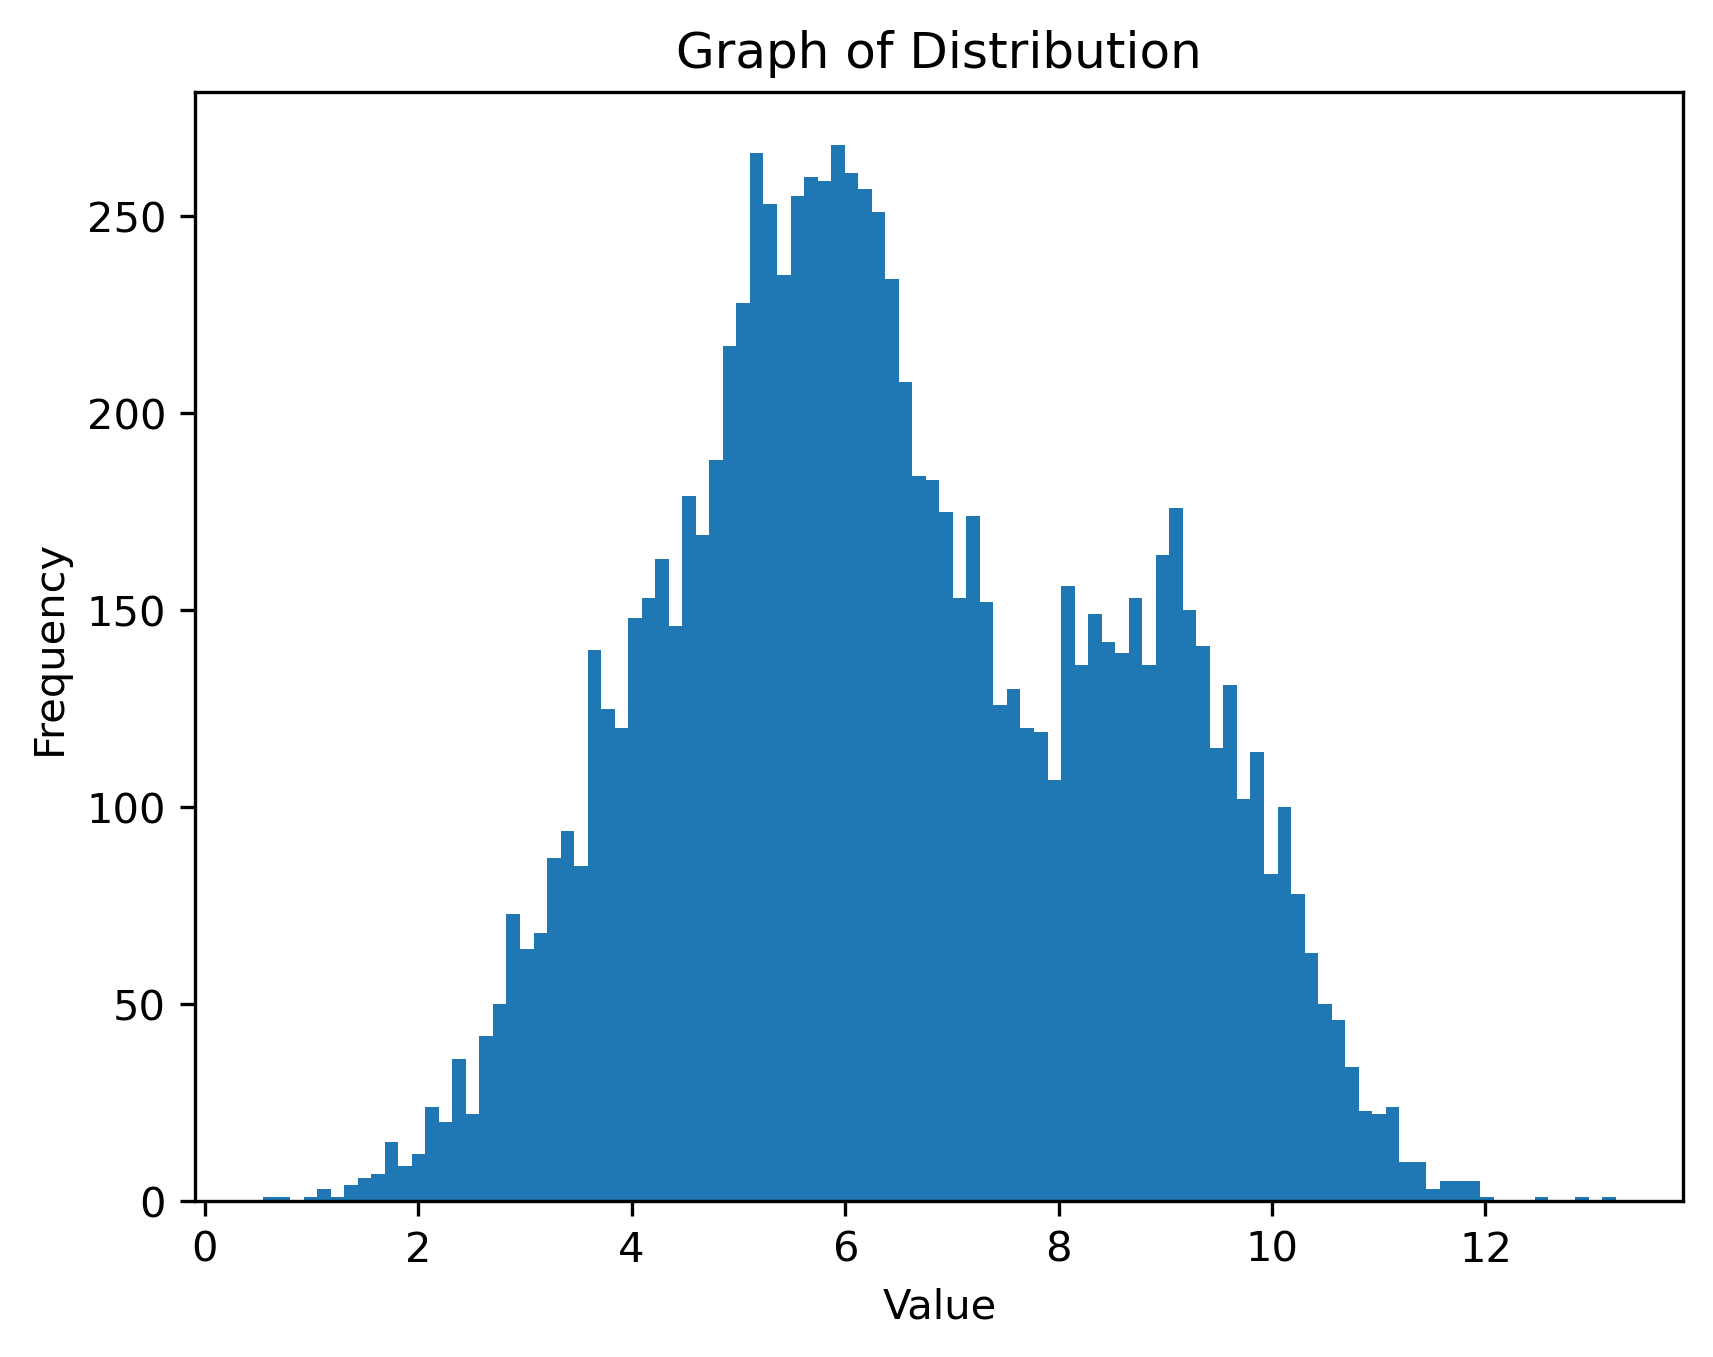
\includegraphics[width=0.5\textwidth]{images/3b.png}
	\caption{Histogram of the data}
\end{figure}
From the above image, we can concluded that the normal distribution parameter $\mu$ is around 6.5
\subsection*{Task C}
\begin{align*}
	\mu_1^{Bin} & = \sum_{i=0}^{N} \binom{n}{i}p^i(1-p)^{n-i} i            \\
	\mu_1^{Bin} & = np \sum_{i=0}^{N} \binom{n-1}{i-1}p^{i-1}(1-p)^{n-i}   \\
	\mu_1^{Bin} & = np                                                     \\
	\mu_2^{Bin} & = \sum_{i=0}^{N} \binom{n}{i}p^i(1-p)^{n-i} i^2          \\
	\mu_2^{Bin} & = np \sum_{i=0}^{N} \binom{n-1}{i-1}p^{i-1}(1-p)^{n-i} i \\
	\mu_2^{Bin} & = np(1-p) + (np)^2
\end{align*}
The parameters found that best fit the data are $n = 20$ and $p = 0.3297$
\begin{figure}
	\centering
	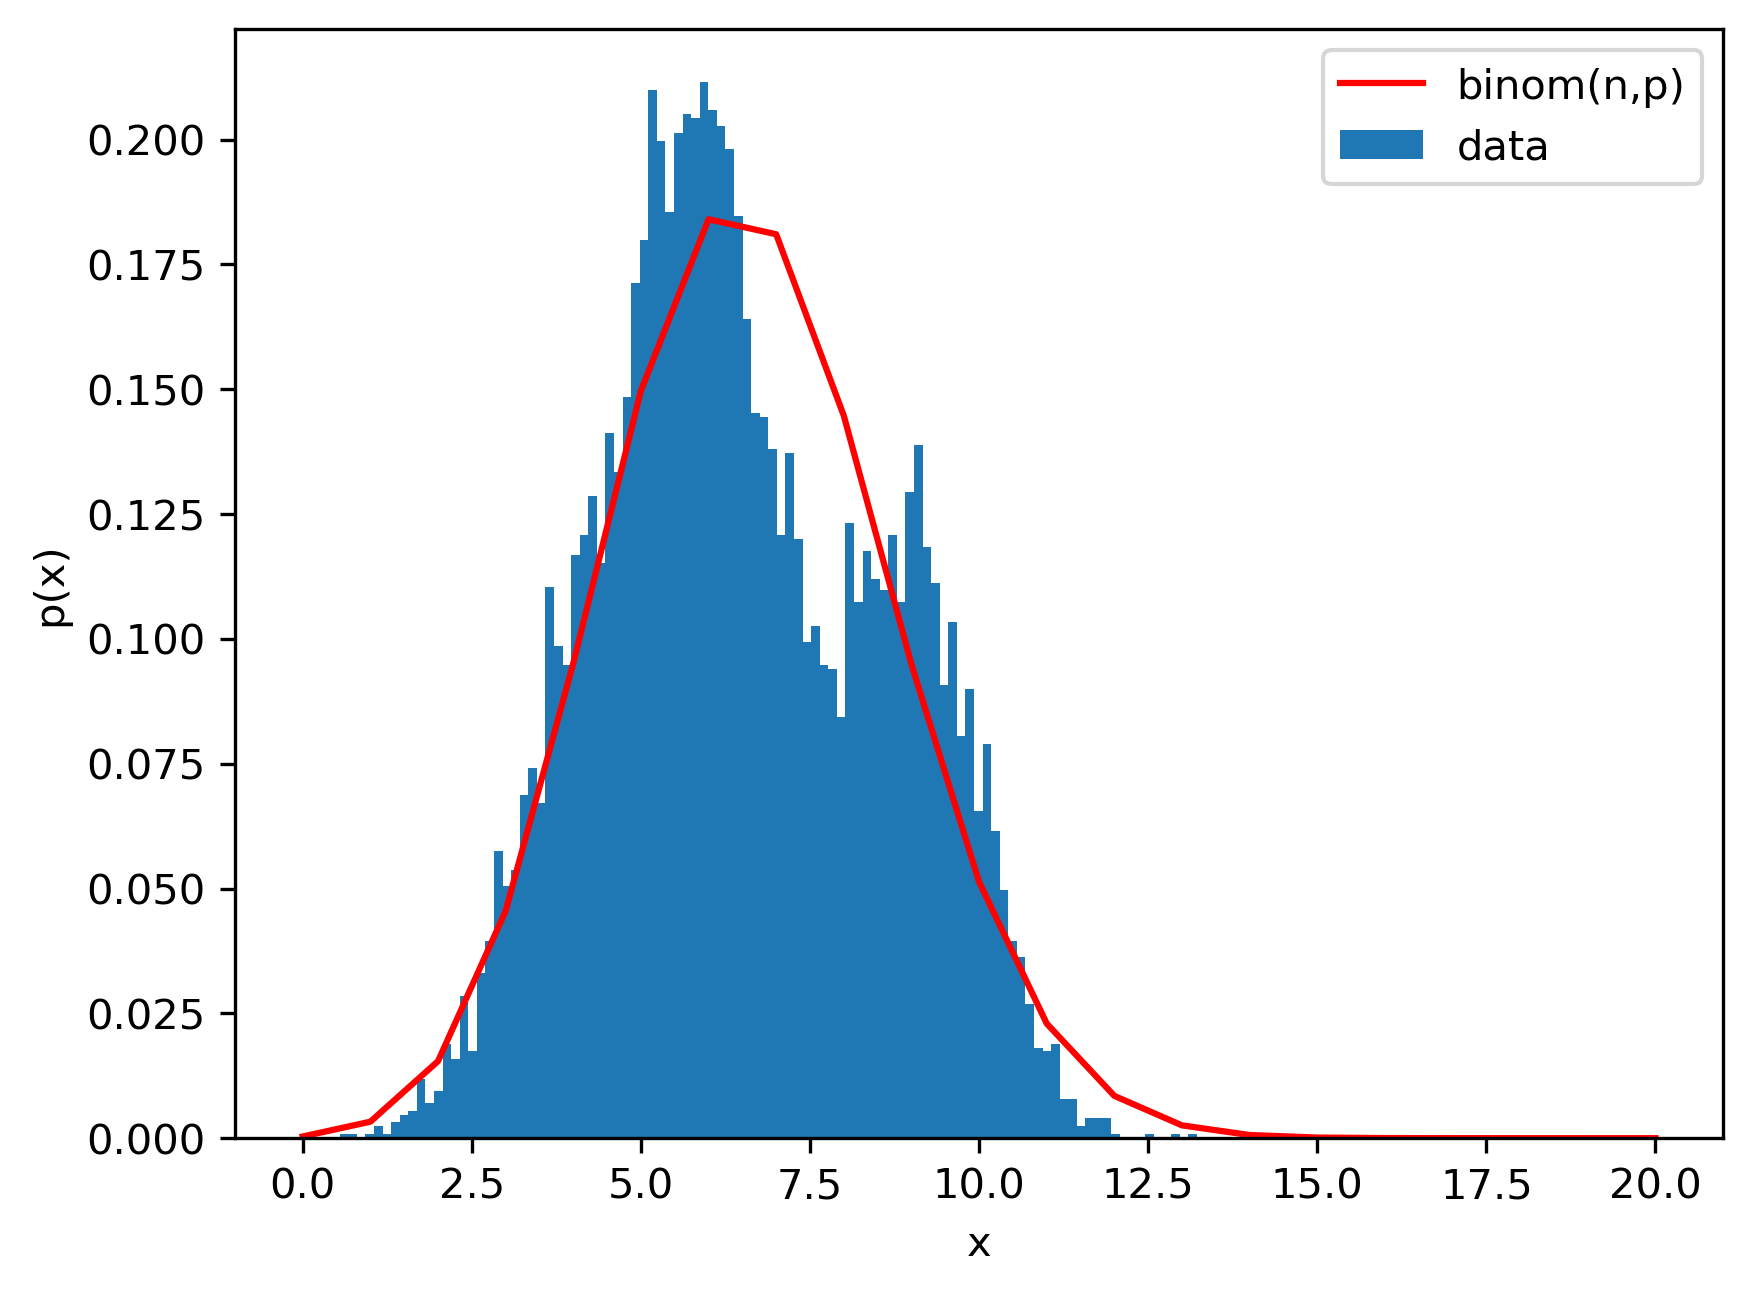
\includegraphics[width=0.5\textwidth]{images/3c.png}
	\caption{Binomial Distribution}
\end{figure}
\subsection*{Task D}
\begin{align*}
	\mu_1^{Gamma} = \int_{0}^{\infty} \frac{1}{\Gamma(k)\theta^k}x^{k}e^{-\frac{x}{\theta}}dx     \\
	\mu_2^{Gamma} = \int_{0}^{\infty} \frac{1}{\Gamma(k)\theta^k}x^{k + 1}e^{-\frac{x}{\theta}}dx \\
\end{align*}
Substituting $x = y\theta$, the integral further simplifies to
\begin{align*}
	\mu_1^{Gamma} = \int_{0}^{\infty} \frac{\theta}{\Gamma(k)}y^{k}e^{-y}dy \\
	\mu_2^{Gamma} = \int_{0}^{\infty} \frac{\theta^2}{\Gamma(k)}y^{k + 1}e^{-y}dy
\end{align*}
The integral is of the form of the gamma function. Using $\Gamma(k+1) = k\Gamma(k)$, we get
\begin{align*}
	\mu_1^{Gamma} = \frac{\theta}{\Gamma(k)}\Gamma(k+1) = \theta k \\
	\mu_2^{Gamma} = \frac{\theta^2}{\Gamma(k)}\Gamma(k+2) = \theta^2 k(k+1)
\end{align*}
Solving the above equations, we get $\theta = 0.67$ and $k = 9.69$
\begin{figure}
	\centering
	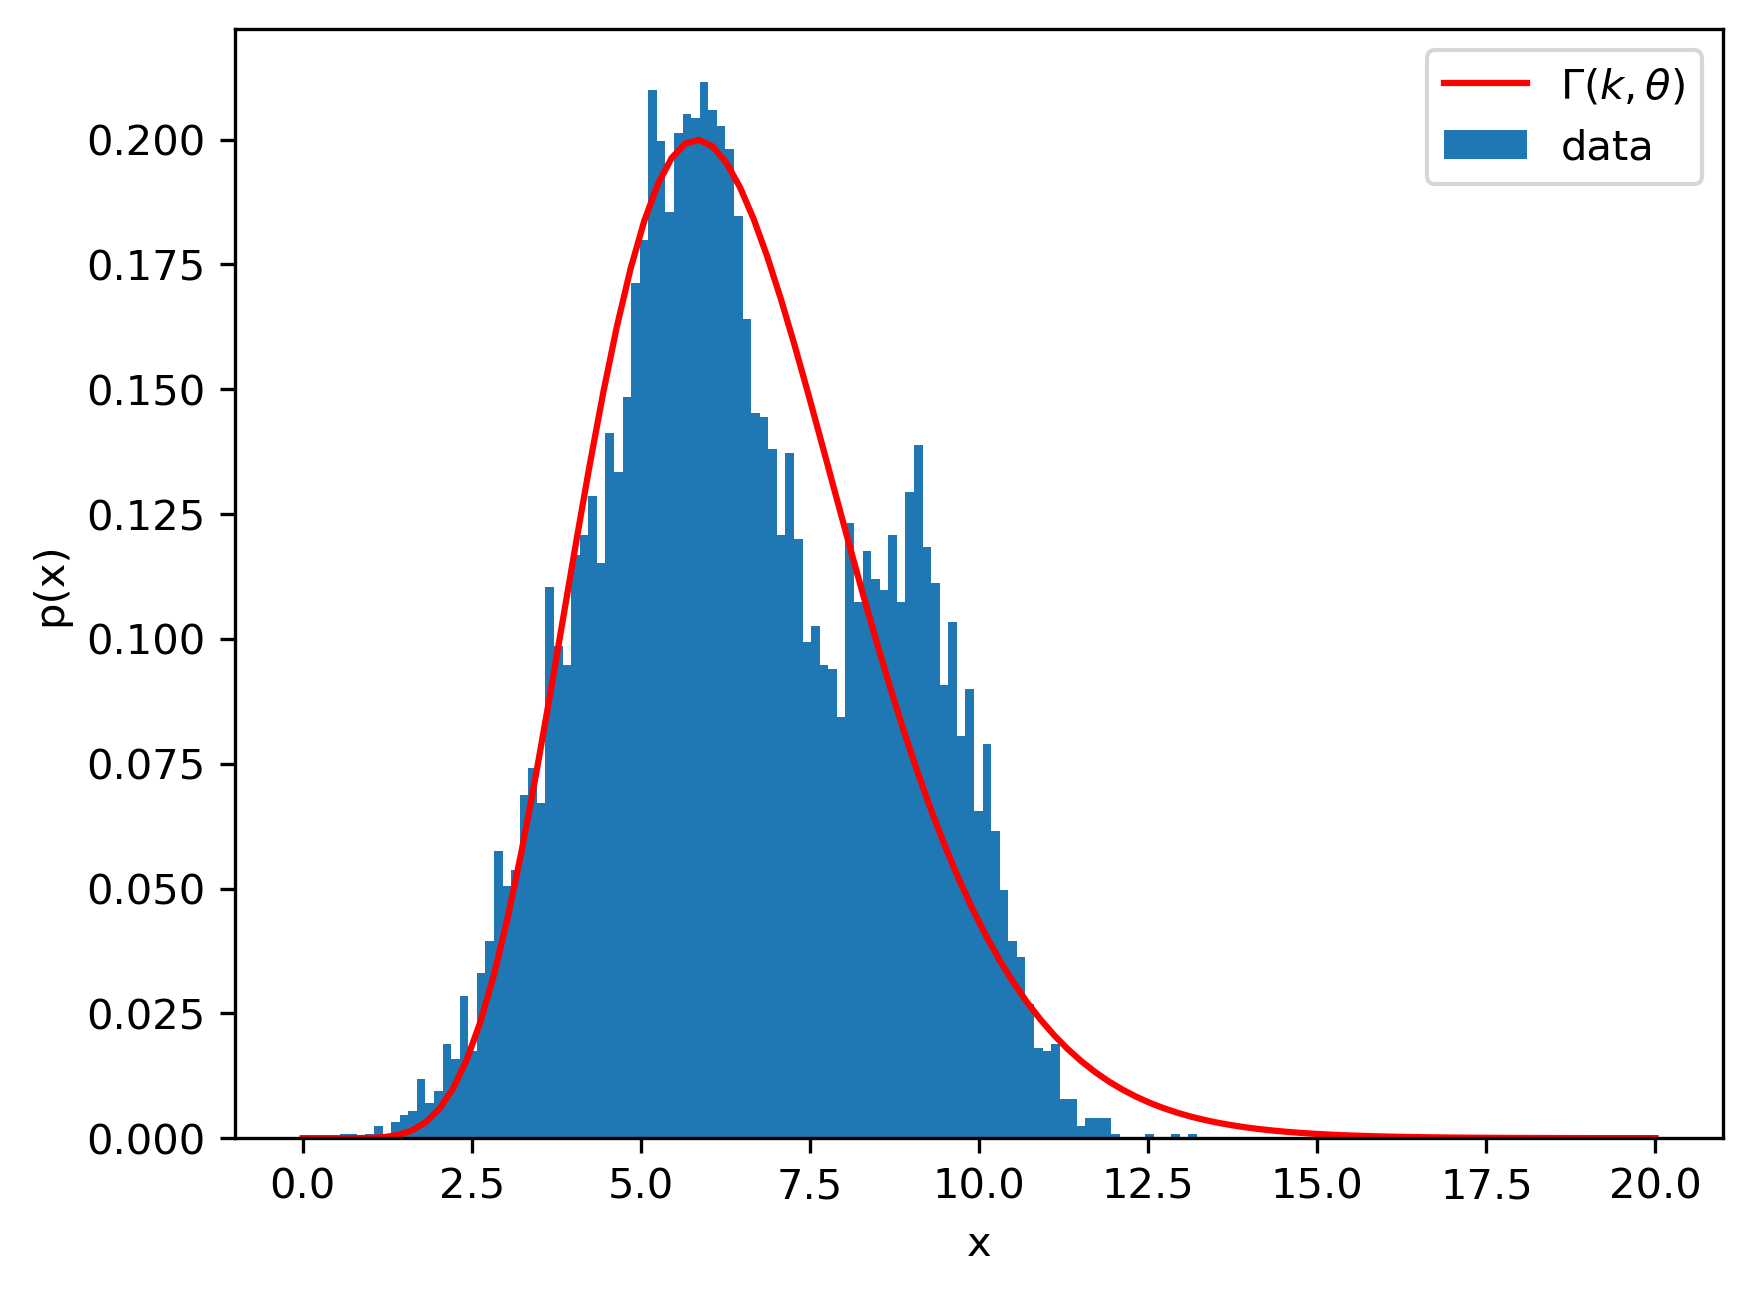
\includegraphics[width=0.5\textwidth]{images/3d.png}
	\caption{Gamma Distribution}
\end{figure}
\subsection*{Task E}
Average Log-likelihood of the binomial distribution: $-2.157$ \\
Average Log likelihood of the gamma distribution: $-2.161$ \\
By comparing the log-likelihoods, we can conclude that the binomial distribution is a better fit for the data.
\subsection*{Task F}
Solving the equations given in the assignment sheet, we get $p_1 = 0.612, p_2 = 0.382, \mu_1^{gmm} = 5.13, \mu_2^{gmm} = 8.774$.\\
Average negative log-likelihood of the Gaussian Mixture Model is $-2.183$.\\
The Gaussian Mixture Model is a worse fit for the data.
\begin{figure}
	\centering
	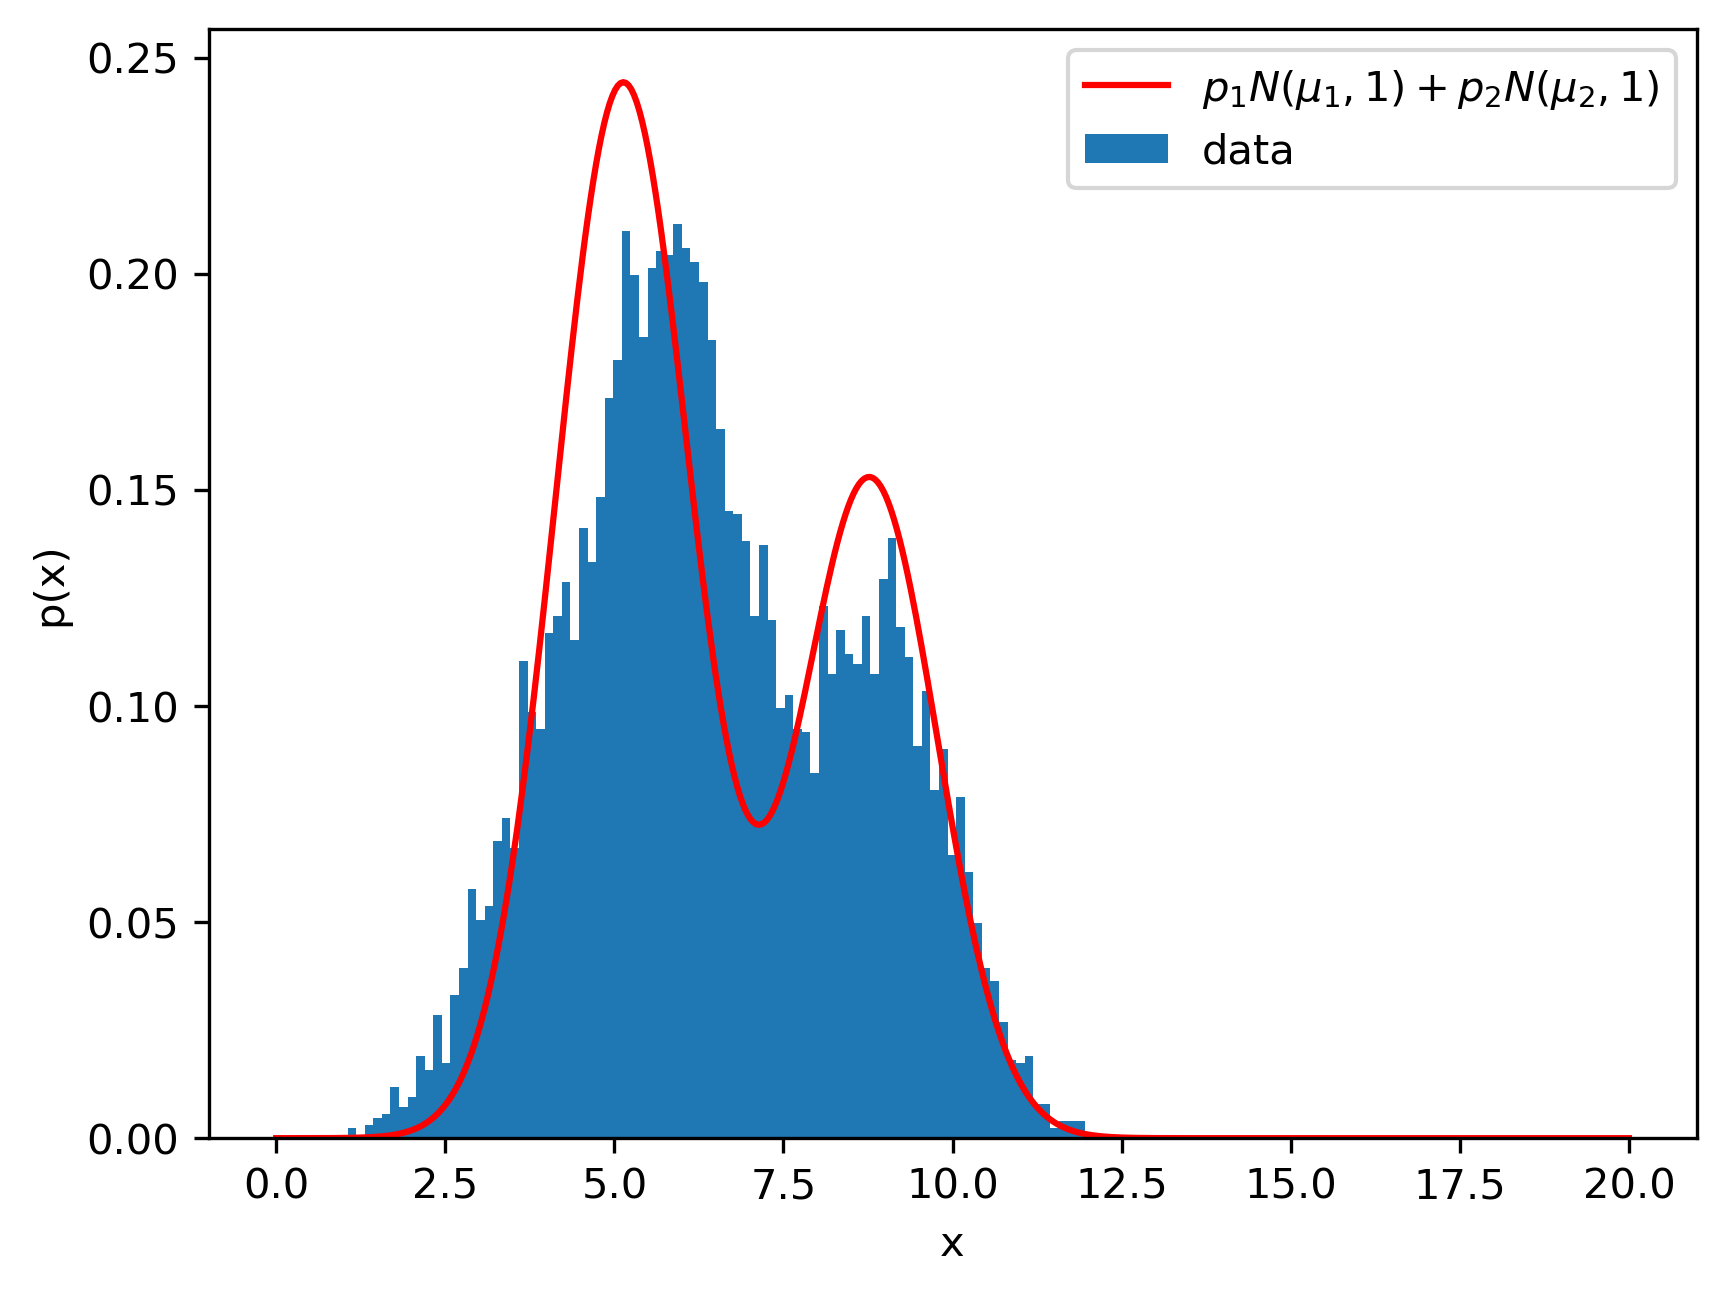
\includegraphics[width=0.5\linewidth]{images/3f.png}
	\caption{Gaussian Mixture Model}
\end{figure}
\subsection*{Bonus}
We predict that the distribution is a mixture of a Gamma distribution and a Gaussian distribution. There are 2 parameters for the Gaussian distribution, 2 parameters for the Gamma distribution and 1 parameter for the mixing proportion. Thus, there are 5 parameters in total.
